\chapter{传输层}

\section{多路复用与多路分解}

\subsection{传输层}

传输层协议为运行在不同主机上的应用进程之间提供了逻辑通信。在发送端,运输层将应用进程的报文添加传输层首部形成传输层分组,称为报文段(segment),这个过程被称为多路复用(multiplexing)。在接收端,网络层从数据报中提取传输层报文段,并交付给传输层,传输层处理报文段,将数据交付给应用进程,这个过程被称为多路分解(demultiplexing)。\\

应用层可以使用UDP和TCP这两种截然不同的传输层协议。其中UDP提供了一种不可靠、无连接的服务,因此,UDP不能保证一个进程发送的数据能够完整无缺地到达目的进程。而TCP提供了一种可靠的、面向连接的服务,通过使用流量控制、序号、确认和定时器,TCP确保正确地、按序地将数据交付给接收进程。\\

\subsection{无连接的多路复用/多路分解}

一个UDP的socket是由一个二元组进行标识的,该二元组包含了目的IP地址和目的端口号。如果两个UDP报文段来自不同的源IP地址或源端口号,但是具有相同的目的IP和目的端口号,那么这两个报文段将通过相同的socket被发送到相同的目的进程。\\

使用UDP时,当A给B发送的报文段中,源端口号是用作返回地址的一部分。当B回发一个报文段给A时,就需要从A到B的报文段中取值。\\

\begin{figure}[H]
	\centering
	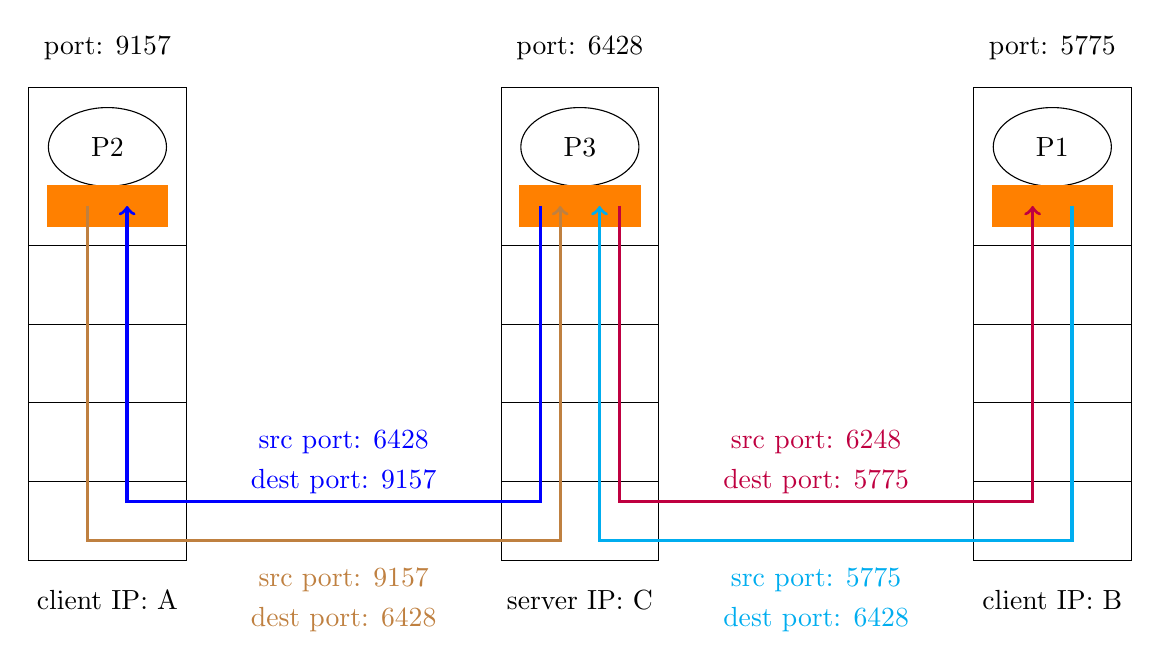
\begin{tikzpicture}
		\draw (1,6.5) node {port: 9157};
		\draw (0,0) rectangle (2,6);
		\draw (0,1) -- (2,1);
		\draw (0,2) -- (2,2);
		\draw (0,3) -- (2,3);
		\draw (0,4) -- (2,4);
		\draw (1,-0.5) node {client IP: A};
		\draw (1,5.25) ellipse (0.75 and 0.5);
		\draw (1,5.25) node {P2};
		\draw[orange, very thick, fill] (0.25,4.25) rectangle (1.75,4.75);

		\draw (7,6.5) node {port: 6428};
		\draw (6,0) rectangle (8,6);
		\draw (6,1) -- (8,1);
		\draw (6,2) -- (8,2);
		\draw (6,3) -- (8,3);
		\draw (6,4) -- (8,4);
		\draw (7,-0.5) node {server IP: C};
		\draw (7,5.25) ellipse (0.75 and 0.5);
		\draw (7,5.25) node {P3};
		\draw[orange, very thick, fill] (6.25,4.25) rectangle (7.75,4.75);

		\draw (13,6.5) node {port: 5775};
		\draw (12,0) rectangle (14,6);
		\draw (12,1) -- (14,1);
		\draw (12,2) -- (14,2);
		\draw (12,3) -- (14,3);
		\draw (12,4) -- (14,4);
		\draw (13,-0.5) node {client IP: B};
		\draw (13,5.25) ellipse (0.75 and 0.5);
		\draw (13,5.25) node {P1};
		\draw[orange, very thick, fill] (12.25,4.25) rectangle (13.75,4.75);

		\draw[->, very thick, brown] (0.75,4.5) -- (0.75,0.25) -- (6.75,0.25) -- (6.75,4.5);
		\draw[brown] (4,-0.25) node {src port: 9157};
		\draw[brown] (4,-0.75) node {dest port: 6428};

		\draw[->, very thick, blue] (6.5,4.5) -- (6.5,0.75) -- (1.25,0.75) -- (1.25,4.5);
		\draw[blue] (4,1.5) node {src port: 6428};
		\draw[blue] (4,1) node {dest port: 9157};

		\draw[->, very thick, cyan] (13.25,4.5) -- (13.25,0.25) -- (7.25,0.25) -- (7.25,4.5);
		\draw[cyan] (10,-0.25) node {src port: 5775};
		\draw[cyan] (10,-0.75) node {dest port: 6428};

		\draw[->, very thick, purple] (7.5,4.5) -- (7.5,0.75) -- (12.75,0.75) -- (12.75,4.5);
		\draw[purple] (10,1.5) node {src port: 6248};
		\draw[purple] (10,1) node {dest port: 5775};
	\end{tikzpicture}
	\caption{无连接的多路复用与多路分解}
\end{figure}

\vspace{0.5cm}

\subsection{面向连接的多路复用与多路分解}

TCP的socket是由一个四元组来标识的,其中包括了源IP地址、源端口号、目的IP地址和目的端口号。与UDP不同的是,两个具有不同源IP地址或源端口号的TCP报文段将被发送到两个不同的socket。\\

\begin{figure}[H]
	\centering
	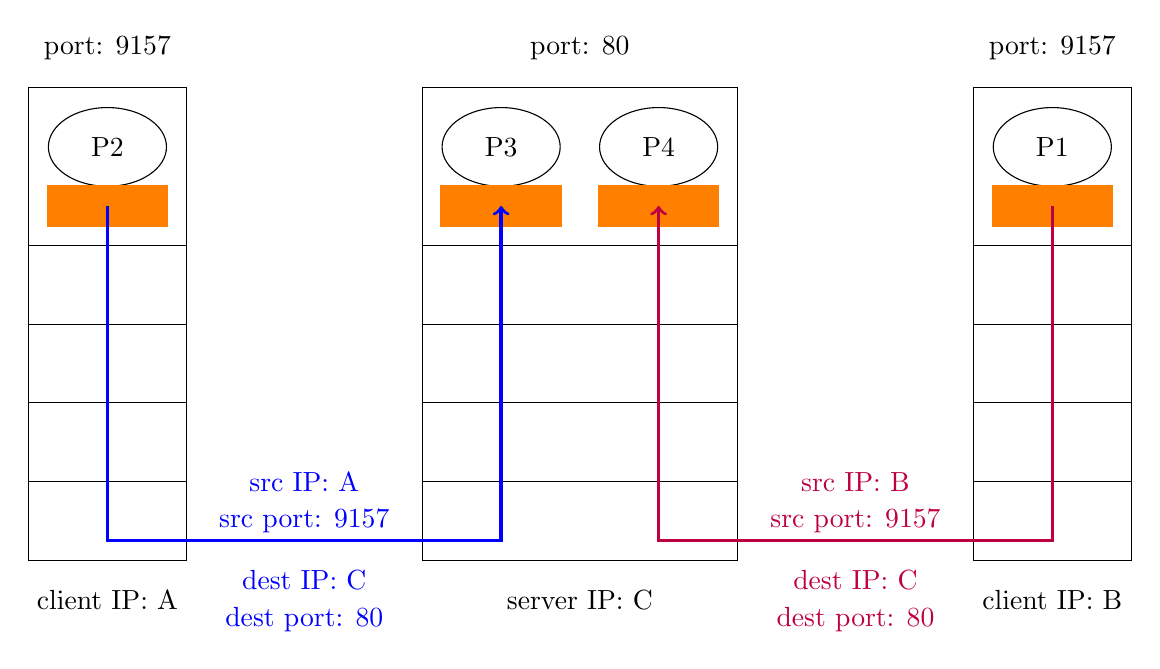
\begin{tikzpicture}
		\draw (1,6.5) node {port: 9157};
		\draw (0,0) rectangle (2,6);
		\draw (0,1) -- (2,1);
		\draw (0,2) -- (2,2);
		\draw (0,3) -- (2,3);
		\draw (0,4) -- (2,4);
		\draw (1,-0.5) node {client IP: A};
		\draw (1,5.25) ellipse (0.75 and 0.5);
		\draw (1,5.25) node {P2};
		\draw[orange, very thick, fill] (0.25,4.25) rectangle (1.75,4.75);

		\draw (7,6.5) node {port: 80};
		\draw (5,0) rectangle (9,6);
		\draw (5,1) -- (9,1);
		\draw (5,2) -- (9,2);
		\draw (5,3) -- (9,3);
		\draw (5,4) -- (9,4);
		\draw (7,-0.5) node {server IP: C};
		\draw (6,5.25) ellipse (0.75 and 0.5);
		\draw (6,5.25) node {P3};
		\draw[orange, very thick, fill] (5.25,4.25) rectangle (6.75,4.75);
		\draw (8,5.25) ellipse (0.75 and 0.5);
		\draw (8,5.25) node {P4};
		\draw[orange, very thick, fill] (7.25,4.25) rectangle (8.75,4.75);

		\draw (13,6.5) node {port: 9157};
		\draw (12,0) rectangle (14,6);
		\draw (12,1) -- (14,1);
		\draw (12,2) -- (14,2);
		\draw (12,3) -- (14,3);
		\draw (12,4) -- (14,4);
		\draw (13,-0.5) node {client IP: B};
		\draw (13,5.25) ellipse (0.75 and 0.5);
		\draw (13,5.25) node {P1};
		\draw[orange, very thick, fill] (12.25,4.25) rectangle (13.75,4.75);

		\draw[->, very thick, blue] (1,4.5) -- (1,0.25) -- (6,0.25) -- (6,4.5);
		\draw[blue] (3.5,1) node {src IP: A};
		\draw[blue] (3.5,0.5) node {src port: 9157};
		\draw[blue] (3.5,-0.25) node {dest IP: C};
		\draw[blue] (3.5,-0.75) node {dest port: 80};

		\draw[->, very thick, purple] (13,4.5) -- (13,0.25) -- (8,0.25) -- (8,4.5);
		\draw[purple] (10.5,1) node {src IP: B};
		\draw[purple] (10.5,0.5) node {src port: 9157};
		\draw[purple] (10.5,-0.25) node {dest IP: C};
		\draw[purple] (10.5,-0.75) node {dest port: 80};
	\end{tikzpicture}
	\caption{面向连接的多路复用与多路分解}
\end{figure}

\newpage

\section{无连接运输UDP}

\subsection{无连接运输UDP}

使用UDP时,在发送报文段之前,发送方和接收方的运输层实体之间没有握手。正因为如此,UDP被称为是无连接的。\\

UDP尽最大努力将数据包交付到目的主机,但不保证可靠性和顺序,也不保证带宽及延迟要求。UDP相较于TCP的优势包括无需连接建立、无连接状态、分组首部开销小。\\

\begin{table}[H]
	\centering
	\begin{tabular}{|p{3cm}<{\centering}|p{3cm}<{\centering}|}
		\hline
		source port \# & dest port \#                    \\
		\hline
		length         & checksum                        \\
		\hline
		\multicolumn{2}{|c|}{application data (message)} \\
		\hline
	\end{tabular}
	\caption{UDP报文段结构}
\end{table}

UDP首部只有4个字段,每个字段由2个字节组成,通过端口号可以将应用数据交给运行在目的端系统中的相应进程。长度字段指示了UDP报文段中的字节数(包括首部)。检验和可以用来检查该报文段中是否出现了差错。\\

\subsection{校验和(Checksum)}

当UDP报文段从源到达目的地的过程中,其中的bit有可能会受到噪声干扰或在路由器中存储而发生改变。UDP检验和提供了差错检测的功能。发送方对UDP报文段中所有内容都当作16位整数进行求和,在求和时遇到的溢出都需要被回卷(wraparound),再对和进行求反,得到的结果被放在UDP报文段中的检验和字段。\\

例如两个16位的整数相加:

\begin{table}[H]
	\centering
	\begin{tabular}{cD{.}{.}{3}}
		  & 1110011001100110  \\
		+ & 1101010101010101  \\
		\hline
		= & 11011101110111011
	\end{tabular}
\end{table}

将溢出位进行回卷:

\begin{table}[H]
	\centering
	\begin{tabular}{cD{.}{.}{3}}
		  & 1011101110111011 \\
		+ & 1                \\
		\hline
		= & 1011101110111100
	\end{tabular}
\end{table}

计算反码得到校验和0100010001000011。\\

接收方收到报文段后,将所有16位整数相加(包括检验和)。如果该分组中没有差错,则计算得到的和将是1111111111111111,否则说明分组中有差错。\\

当检验和错误的时候,该分组一定错误,将会被丢弃。但是当检验和没有错误时,并不能保证分组是完全正确的。虽然UDP提供差错检测,但它对差错恢复无能无力。

\newpage

\section{可靠数据传输}

\subsection{可靠数据传输(RDT, Reliable Data Transfer)}

由于可靠数据传输协议的下层协议也许是不可靠的,信道的不可靠特性决定了可靠数据传输协议的复杂性,例如TCP就是在不可靠的端到端网络层之上实现的可靠数据传输协议。\\

\begin{figure}[H]
	\centering
	\begin{tikzpicture}
		\draw (0,10) node {应用层};
		\draw (0,5) node {传输层};
		\draw (0,0) node {网络层};
		\draw[dashed] (0,7.5) -- (14,7.5);
		\draw[dashed] (0,2.5) -- (14,2.5);

		\draw (2,12) rectangle (3,13);
		\draw (5,12) rectangle (6,13);
		\draw (8,12) rectangle (9,13);
		\draw (11,12) rectangle (12,13);

		\draw (2.5,10) ellipse (0.75 and 0.5);
		\draw (2.5,10) node {发送};
		\draw (5.5,10) ellipse (0.75 and 0.5);
		\draw (5.5,10) node {接收};

		\node at (4.3,5) [cylinder, shape border rotate=180, draw, minimum height=2.5cm, minimum width=1cm]{可靠信道};
		\draw[->, very thick] (2.5,9.5) -- (2.5,5) -- (3,5);
		\draw[->, very thick] (5.4,5) -- (5.5,5) -- (5.5,9.5);

		\node at (10.3,0) [cylinder, shape border rotate=180, draw, minimum height=2.5cm, minimum width=1cm]{不可靠信道};
		\draw (7.5,4.5) rectangle (9.5,5.5);
		\draw (8.5,5) node {rdt};
		\draw (10.5,4.5) rectangle (12.5,5.5);
		\draw (11.5,5) node {rdt};

		\draw[->, very thick] (8.5,9) -- (8.5,5.5);
		\draw[->, very thick] (8.5,4.5) -- (8.5,0) -- (8.8,0);
		\draw[->, very thick] (11.5,0) -- (11.5,4.5);
		\draw[->, very thick] (11.5,5.5) -- (11.5,9);

		\draw (7,6.5) node {rdt\_send()};
		\draw (7,3.5) node {udt\_send()};
		\draw (13,6.5) node {deliver\_data()};
		\draw (13,3.5) node {udt\_rcv()};
	\end{tikzpicture}
	\caption{可靠数据传输}
\end{figure}

\vspace{0.5cm}

\subsection{rdt 1.0:经完全可靠信道的可靠数据传输}

考虑最简单的情况,假设底层信道是完全可靠的(不会出错、不会丢失)。有限状态机(FSM, Finite State Machine)可以用于描述发送方和接收方的操作。\\

\begin{figure}[H]
	\centering
	\begin{tikzpicture}
		\node[state, initial, draw, align=center] (s1) {wait for\\call};
		\draw (s1) edge[loop right] node{} (s1);
		\draw (5,0.5) node {rdt\_send(data)};
		\draw (2.5,0.25) -- (7.5,0.25);
		\draw (5,0) node {pkt = make\_pkt(data)};
		\draw (4.25,-0.5) node {udt\_send(pkt)};
	\end{tikzpicture}
	\caption{rdt 1.0发送端}
\end{figure}

\vspace{0.5cm}

\begin{figure}[H]
	\centering
	\begin{tikzpicture}
		\node[state, initial, draw, align=center] (s1) {wait for\\call};
		\draw (s1) edge[loop right] node{} (s1);
		\draw (5.5,0.5) node {rdt\_rcv(pkt)};
		\draw (3,0.25) -- (8,0.25);
		\draw (5.3,0) node {data = extract(pkt)};
		\draw (5.2,-0.5) node {deliver\_data(data)};
	\end{tikzpicture}
	\caption{rdt 1.0接收端}
\end{figure}

\vspace{0.5cm}

\subsection{rdt 2.0:经具有比特差错信道的可靠数据传输}

在分组的传输、传播或缓存的过程中,分组中的比特可能会受损。类似于打电话,当接听电话的人听到并理解一句话时会说“OK”,但如果没听清,就会要求对方再说一遍。\\

rdt 2.0增加了差错检验、接收方反馈和重传机制。当接收方接收到正确的报文时,就给对方一个肯定确认(ACK, positive acknowledgment),告诉他“没问题”。当接收方检测到报文错误时,就需要给对方一个否定确认(NAK, negative acknowledgment),告诉对方“你给我发的不对,重新给我发一份新的吧”。\\

\begin{figure}[H]
	\centering
	\begin{tikzpicture}[node distance=5cm]
		\node[state, initial, draw, align=center] (s1) {wait for\\call};
		\node[state, right of=s1, draw, align=center] (s2) {wait for\\ACK/NAK};

		\draw[->] (s1) edge[above, bend left] node{} (s2);
		\draw[->] (s2) edge[above, bend left] node{} (s1);
		\draw[->] (s2) edge[loop right] node{} (s2);

		\draw (0,3) node {rdt\_send(data)};
		\draw (-2.5,2.75) -- (2.5,2.75);
		\draw (0,2.5) node {sndpkt = make\_pkt(data)};
		\draw (-0.8,2) node {udt\_send(sndpkt)};

		\draw (9,2) node {rdt\_rcv(rcvpkt) \&\& is\_nak(rcvpkt)};
		\draw (5.5,1.75) -- (12.5,1.75);
		\draw (9,1.5) node {udt\_send(sndpkt)};

		\draw (3,-2) node {rdt\_rcv(rcvpkt) \&\& is\_ack(rcvpkt)};
		\draw (-0.5,-2.25) -- (6.5,-2.25);
		\draw (3,-2.5) node {$ \wedge $};
	\end{tikzpicture}
	\caption{rdt 2.0发送端}
\end{figure}

\vspace{0.5cm}

\begin{figure}[H]
	\centering
	\begin{tikzpicture}
		\node[state, initial, draw, align=center] (s1) {wait for\\call};
		\draw (s1) edge[loop above] node{} (s1);
		\draw (s1) edge[loop below] node{} (s1);

		\draw (4,3) node {rdt\_rcv(rcvpkt) \&\& corrupt(rcvpkt)};
		\draw (0.5,2.75) -- (7.5,2.75);
		\draw (3.5,2.5) node {sndpkt = make\_pkt(NAK)};
		\draw (2.65,2) node {udt\_send(sndpkt)};

		\draw (4,-1.5) node {rdt\_rcv(rcvpkt) \&\& !corrupt(rcvpkt)};
		\draw (0.5,-1.75) -- (7.5,-1.75);
		\draw (3.5,-2) node {data = extract(rcvpkt)};
		\draw (3.15,-2.5) node {deliver\_data(data)};
		\draw (3.95,-3) node {sndpkt = make\_pkt(ACK)};
		\draw (3.1,-3.5) node {udt\_send(sndpkt)};
	\end{tikzpicture}
	\caption{rdt 2.0接收端}
\end{figure}

\vspace{0.5cm}

发送方在将分组发送后,等待来自接收方的ACK或NAK。如果收到ACK,则代表接收方正确地接收了分组,那么就回到初始状态继续等待上层的数据。如果收到NAK,那就表示接收方没有收到正确的分组,需要进行重传并且继续处于等待ACK或NAK的状态。像这种只有当发送方接收到ACK后才能够继续发送新的报文的协议,被称为停等协议(stop-and-wait)。\\

rdt 2.0看起来似乎可以运行了,但遗憾的是,它存在一个致命的缺陷——ACK或NAK也存在受损的可能性!\\

当发送方收到的是一个受损的ACK或NAK时,如果发送方简单地选择直接重发分组会导致接收方收到重复的分组。\\

\subsection{rdt 2.1:带序号消息协议}

发送方可以为分组添加序号,接收方只需检查需要就可确定收到的分组是否重复。对于停等协议而言,序号只需要使用0和1就可以了。\\

\begin{figure}[H]
	\centering
	\begin{tikzpicture}[node distance=5cm]
		\node[state, initial, draw, align=center] (s1) {wait for\\call 0};
		\node[state, right of=s1, draw, align=center] (s2) {wait for\\ACK/NAK 0};
		\node[state, below of=s2, draw, align=center] (s3) {wait for\\call 1};
		\node[state, left of=s3, draw, align=center] (s4) {wait for\\ACK/NAK 1};

		\draw[->] (s1) edge[above, bend left] node{} (s2);
		\draw[->] (s2) edge[loop right] node{} (s2);
		\draw[->] (s2) edge[above, bend left] node{} (s3);
		\draw[->] (s3) edge[above, bend left] node{} (s4);
		\draw[->] (s4) edge[loop left] node{} (s4);
		\draw[->] (s4) edge[above, bend left] node{} (s1);

		\draw (3,3) node {rdt\_send(data)};
		\draw (0,2.75) -- (6,2.75);
		\draw (3,2.5) node {sndpkt = make\_pkt(0, data)};
		\draw (2,2) node {udt\_send(sndpkt)};

		\draw (8.5,2.5) node {rdt\_rcv(rcvpkt) \&\&};
		\draw (8.3,2) node {(corrupt(rcvpkt) ||};
		\draw (8.1,1.5) node {is\_nak(rcvpkt))};
		\draw (6.5,1.25) -- (10.5,1.25);
		\draw (8.5,1) node {udt\_send(sndpkt)};

		\draw (8,-2) node {rdt\_rcv(rcvpkt) \&\&};
		\draw (8,-2.5) node {!corrupt(rcvpkt) \&\&};
		\draw (7.6,-3) node {is\_ack(rcvpkt))};
		\draw (6,-3.25) -- (10,-3.25);
		\draw (7.5,-3.5) node {$ \wedge $};

		\draw (4,-7) node {rdt\_send(data)};
		\draw (1,-7.25) -- (7,-7.25);
		\draw (4,-7.5) node {sndpkt = make\_pkt(1, data)};
		\draw (3,-8) node {udt\_send(sndpkt)};

		\draw (-2,-7) node {rdt\_rcv(rcvpkt) \&\&};
		\draw (-2.2,-7.5) node {(corrupt(rcvpkt) ||};
		\draw (-2.4,-8) node {is\_nak(rcvpkt))};
		\draw (-4,-8.25) -- (0,-8.25);
		\draw (-2,-8.5) node {udt\_send(sndpkt)};

		\draw (-3,-2) node {rdt\_rcv(rcvpkt) \&\&};
		\draw (-3,-2.5) node {!corrupt(rcvpkt) \&\&};
		\draw (-3.4,-3) node {is\_ack(rcvpkt))};
		\draw (-5,-3.25) -- (-1,-3.25);
		\draw (-3,-3.5) node {$ \wedge $};
	\end{tikzpicture}
	\caption{rdt 2.1发送端}
\end{figure}

\vspace{0.5cm}

\begin{figure}[H]
	\centering
	\begin{tikzpicture}[node distance=5cm]
		\node[state, initial, draw, align=center] (s1) {wait for\\call 0};
		\node[state, right of=s1, draw, align=center] (s2) {wait for\\call 1};

		\draw[->] (s1) edge[above, bend left] node{} (s2);
		\draw[->] (s2) edge[above, bend left] node{} (s1);
		\draw[->] (s1) edge[loop above] node{} (s1);
		\draw[->] (s1) edge[loop below] node{} (s1);
		\draw[->] (s2) edge[loop above] node{} (s2);
		\draw[->] (s2) edge[loop below] node{} (s2);

		\draw (2.5,5) node {rdt\_rcv(rcvpkt) \&\&};
		\draw (2.5,4.5) node {!corrupt(rcvpkt) \&\&};
		\draw (2.2,4) node {has\_seq0(rcvpkt)};
		\draw (0.3,3.75) -- (5.7,3.75);
		\draw (2.6,3.5) node {data = extract(rcvpkt)};
		\draw (2.25,3) node {deliver\_data(data)};
		\draw (3,2.5) node {sndpkt = make\_pkt(ACK)};
		\draw (2.2,2) node {udt\_send(sndpkt)};

		\draw (-3.4,3) node {rdt\_rcv(rcvpkt) \&\&};
		\draw (-3.85,2.5) node {corrupt(rcvpkt)};
		\draw (-5.5,2.25) -- (-0.3,2.25);
		\draw (-2.75,2) node {sndpkt = make\_pkt(NAK)};
		\draw (-3.6,1.5) node {udt\_send(sndpkt)};

		\draw (-3.5,-2) node {rdt\_rcv(rcvpkt) \&\&};
		\draw (-3.5,-2.5) node {!corrupt(rcvpkt) \&\&};
		\draw (-3.7,-3) node {has\_seq1(rcvpkt)};
		\draw (-5.5,-3.25) -- (-0.3,-3.25);
		\draw (-2.8,-3.5) node {sndpkt = make\_pkt(ACK)};
		\draw (-3.65,-4) node {udt\_send(sndpkt)};

		\draw (2.5,-2) node {rdt\_rcv(rcvpkt) \&\&};
		\draw (2.5,-2.5) node {!corrupt(rcvpkt) \&\&};
		\draw (2.2,-3) node {has\_seq1(rcvpkt)};
		\draw (0.3,-3.25) -- (5.7,-3.25);
		\draw (2.6,-3.5) node {data = extract(rcvpkt)};
		\draw (2.25,-4) node {deliver\_data(data)};
		\draw (3,-4.5) node {sndpkt = make\_pkt(ACK)};
		\draw (2.2,-5) node {udt\_send(sndpkt)};

		\draw (7.7,3) node {rdt\_rcv(rcvpkt) \&\&};
		\draw (7.2,2.5) node {corrupt(rcvpkt)};
		\draw (5.5,2.25) -- (11,2.25);
		\draw (8.3,2) node {sndpkt = make\_pkt(NAK)};
		\draw (7.45,1.5) node {udt\_send(sndpkt)};

		\draw (8,-2) node {rdt\_rcv(rcvpkt) \&\&};
		\draw (8,-2.5) node {!corrupt(rcvpkt) \&\&};
		\draw (7.75,-3) node {has\_seq0(rcvpkt)};
		\draw (6,-3.25) -- (11.25,-3.25);
		\draw (8.65,-3.5) node {sndpkt = make\_pkt(ACK)};
		\draw (7.8,-4) node {udt\_send(sndpkt)};
	\end{tikzpicture}
	\caption{rdt 2.1接收端}
\end{figure}

\vspace{0.5cm}

\subsection{rdt 2.2:无NAK消息协议}

rdt 2.2与同rdt 2.1的功能相同,但是只使用ACK。接收方每次ACK最后一个被正确接收的分组,当发送方收到重复的ACK之后,采用与NAK相同的处理动作,将分组重传给接收方。\\

\begin{figure}[H]
	\centering
	\begin{tikzpicture}[node distance=4cm]
		\node[state, initial, draw, align=center] (s1) {wait for\\call 0};
		\node[state, right of=s1, draw, align=center] (s2) {wait for\\ACK 0};
		\node[state, below of=s2, draw, align=center] (s3) {wait for\\call 1};
		\node[state, left of=s3, draw, align=center] (s4) {wait for\\ACK 1};

		\draw[->] (s1) edge[above, bend left] node{} (s2);
		\draw[->] (s2) edge[loop right] node{} (s2);
		\draw[->] (s2) edge[above, bend left] node{} (s3);
		\draw[->] (s3) edge[above, bend left] node{} (s4);
		\draw[->] (s4) edge[loop left] node{} (s4);
		\draw[->] (s4) edge[above, bend left] node{} (s1);

		\draw (3,3) node {rdt\_send(data)};
		\draw (0,2.75) -- (6,2.75);
		\draw (3,2.5) node {sndpkt = make\_pkt(0, data)};
		\draw (2,2) node {udt\_send(sndpkt)};

		\draw (8.5,2.5) node {rdt\_rcv(rcvpkt) \&\&};
		\draw (8.3,2) node {(corrupt(rcvpkt) ||};
		\draw (8.3,1.5) node {is\_ack(rcvpkt, 1))};
		\draw (6.5,1.25) -- (10.5,1.25);
		\draw (8.5,1) node {udt\_send(sndpkt)};

		\draw (8,-1.5) node {rdt\_rcv(rcvpkt) \&\&};
		\draw (8,-2) node {!corrupt(rcvpkt) \&\&};
		\draw (7.9,-2.5) node {is\_ack(rcvpkt, 0))};
		\draw (6,-2.75) -- (10,-2.75);
		\draw (7.5,-3) node {$ \wedge $};

		\draw (4,-6) node {rdt\_send(data)};
		\draw (1,-6.25) -- (7,-6.25);
		\draw (4,-6.5) node {sndpkt = make\_pkt(1, data)};
		\draw (3,-7) node {udt\_send(sndpkt)};

		\draw (-2,-5.5) node {rdt\_rcv(rcvpkt) \&\&};
		\draw (-2.2,-6) node {(corrupt(rcvpkt) ||};
		\draw (-2.2,-6.5) node {is\_ack(rcvpkt, 0))};
		\draw (-4,-6.75) -- (0,-6.75);
		\draw (-2,-7) node {udt\_send(sndpkt)};

		\draw (-3,-1.5) node {rdt\_rcv(rcvpkt) \&\&};
		\draw (-3,-2) node {!corrupt(rcvpkt) \&\&};
		\draw (-3.2,-2.5) node {is\_ack(rcvpkt, 1))};
		\draw (-5,-2.75) -- (-1,-2.75);
		\draw (-3,-3) node {$ \wedge $};
	\end{tikzpicture}
	\caption{rdt 2.2发送端}
\end{figure}

\vspace{0.5cm}

\begin{figure}[H]
	\centering
	\begin{tikzpicture}[node distance=5cm]
		\draw[->] (-1,2) -- (-0.6,0.9);
		\draw (-1.5,1.5) node {start};

		\node[state, draw, align=center] (s1) {wait for\\call 0};
		\node[state, right of=s1, draw, align=center] (s2) {wait for\\call 1};

		\draw[->] (s1) edge[above, bend left] node{} (s2);
		\draw[->] (s2) edge[above, bend left] node{} (s1);
		\draw[->] (s1) edge[loop left] node{} (s1);
		\draw[->] (s2) edge[loop right] node{} (s2);

		\draw (1.8,5) node {rdt\_rcv(rcvpkt) \&\&};
		\draw (1.8,4.5) node {!corrupt(rcvpkt) \&\&};
		\draw (1.5,4) node {has\_seq0(rcvpkt)};
		\draw (-0.4,3.75) -- (5.5,3.75);
		\draw (1.9,3.5) node {data = extract(rcvpkt)};
		\draw (1.55,3) node {deliver\_data(data)};
		\draw (2.55,2.5) node {sndpkt = make\_pkt(ACK, 0)};
		\draw (1.5,2) node {udt\_send(sndpkt)};

		\draw (-3.5,-1) node {rdt\_rcv(rcvpkt) \&\&};
		\draw (-3.5,-1.5) node {(corrupt(rcvpkt) \&\&};
		\draw (-3.7,-2) node {has\_seq1(rcvpkt))};
		\draw (-5.5,-2.25) -- (0.5,-2.25);
		\draw (-2.65,-2.5) node {sndpkt = make\_pkt(ACK, 1)};
		\draw (-3.7,-3) node {udt\_send(sndpkt)};

		\draw (2.7,-1.5) node {rdt\_rcv(rcvpkt) \&\&};
		\draw (2.7,-2) node {!corrupt(rcvpkt) \&\&};
		\draw (2.4,-2.5) node {has\_seq1(rcvpkt)};
		\draw (0.5,-2.75) -- (5.9,-2.75);
		\draw (2.8,-3) node {data = extract(rcvpkt)};
		\draw (2.45,-3.5) node {deliver\_data(data)};
		\draw (3.4,-4) node {sndpkt = make\_pkt(ACK, 1)};
		\draw (2.4,-4.5) node {udt\_send(sndpkt)};

		\draw (7.7,3.5) node {rdt\_rcv(rcvpkt) \&\&};
		\draw (7.5,3) node {(corrupt(rcvpkt) ||};
		\draw (7.5,2.5) node {has\_seq0(rcvpkt))};
		\draw (5.5,2.25) -- (11.5,2.25);
		\draw (8.5,2) node {sndpkt = make\_pkt(ACK, 0)};
		\draw (7.45,1.5) node {udt\_send(sndpkt)};
	\end{tikzpicture}
	\caption{rdt 2.2接收端}
\end{figure}

\vspace{0.5cm}

\subsection{rdt 3.0:经具有比特差错的丢包信道的可靠数据传输}

